\section{Blockchain: Technical Primer} \label{Blockchain}
This chapter explains some of the technical concepts and terminologies related to blockchain. This technology allows participants to transact with each other using a peer-to-peer network that guarantees censorship resistance, immutability, transaction finality, and protection against double spend attacks. In order to better explain how it works consider figure [\ref{fig:bc-workflow}]. Alice wants to transfer two bitcoins to Bob. She uses her private key to creates a signed transaction for transferring these coins to Bob. Every user in the network has pair of keys; a public key that serves as their unique identifier or address and a private key for signing transactions see section [\ref{AC}]. The signed transaction is broadcast to the bitcoin network where it waits until it is picked up by a special node called a miner. The miner verifies transaction signatures and batches pending transactions into blocks. Each block carries the hash of the one that came immediately before it. Next step is to calculate the hash of the entire block and append it at the end of the blockchain see figure [\ref{fig:bc-workflow}]. Blockchain protocols have built in consensus mechanism to ensure that peers always agree on only one longest chain see section [\ref{Mining}]. Blockchain is not just a technology it is actually a systems and like most systems it is composed of individual components which come together to make the whole. The next few sections explain the important building blocks or sub components of the blockchain system.

\begin{figure}[t]
	\centering
    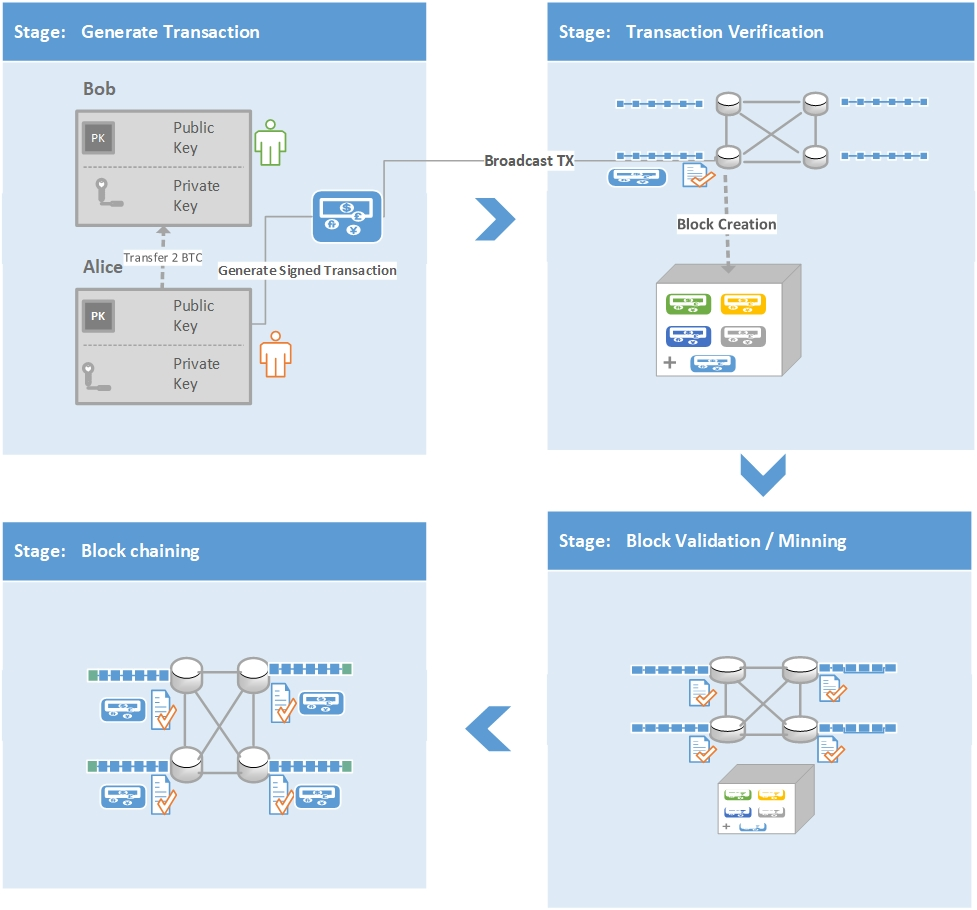
\includegraphics[width=160mm,scale=1]{figs/bc-workflow}
	\caption{How does blockchain work?}
	\label{fig:bc-workflow}
\end{figure}
\clearpage

\subsection{Distributed Ledger Technology} 
Distributed ledger Technology refers to a shared and distributed database replicated across members of a peer-to-peer network. Each member of the network receives the same copy of the data. New data can only be added to the ledger when consensus is achieved among the members. Consensus rules and mechanisms [\ref{Mining}] may vary from network to network. These rules are designed to ensure that data on the ledger remains synchronized across network participants. Blockchain is a special type of distributed ledger where cryptography is used to achieve consensus and ensure transaction authenticity.  Information stored on the blockchain is immutable i.e. once recorded it cannot be altered. Blockchain is not the only structure used for DLT. IOTA \cite{wiki:003} and Hashgraph have successfully employed Directed Acyclic Graphs (DAG) \cite{wiki:002} for creating their DLT. 
\subsection{Asymmetric Cryptography} \label{AC}
Asymmetric or public key cryptography is an important building block of any blockchain network. This cryptography technique relies on a pair of keys: A public key which is widely available or shared with everyone, and a private key which is only known to the owner. These two keys are mathetimatically related to each other in that one key usually encrypts and the other key is used for decryption. If the private key encrypts only the corresponding public key can decrypt and vice versa \cite{wiki:004}. Public key cryptography is widely employed for:

\textbf{Public key Encryption:} is an encryption technique where data is encrypted using senders public key. The recipient can only decrypt the data and read the message if he is in possession of the corresponding private key.

\textbf{Digital Signatures:} based on public key cryptography are used in a number of applications including blockchain. Data or message is signed with sender’s private key. Anyone can verify the message signature using the corresponding public key. In Bitcoin, Ethereum and other blockchain networks digital signatures are used to guarantee authenticity, integrity and non-repudiation.
\subsubsection{Digital Wallets}
In cryptocurrency applications we often hear the term digital wallets. It is a program which shows users account balance and helps them transfer coins to other users. In essence a digital wallet is the private key of that user. It provides additional functionalities like signing transactions for transferring coins, and querying the blockchain to get the cryptocurrency balance associated with their private key.  Figure [\ref{fig:bc-sig}] shows how digital signatures are used in the blockchain. 

\begin{figure}[h]
	\centering
    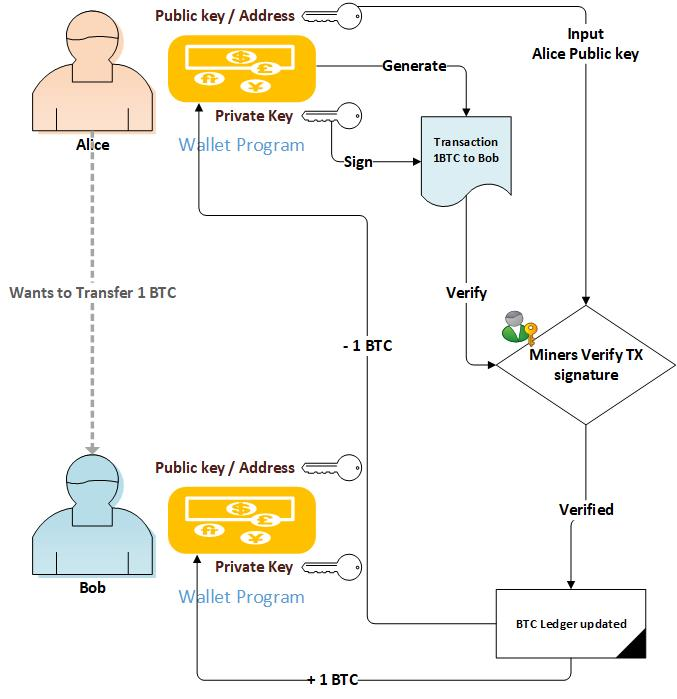
\includegraphics[width=160mm,scale=1]{figs/sig}
	\caption{Digital Signatures in Blockchain}
	\label{fig:bc-sig}
\end{figure}
\clearpage

\subsection{Hashing}
Hashing is used to calculate fixed length hashes for variable length data. Hashing algorithms are designed in a way that even a slight change in the input data will result in a vastly different output hash. All cryptocurrency networks use some sort of hashing algorithms in their mining [\ref{Mining}] process. Ethereum uses an algorithm called Ethash (modfied Dagger Hashimoto) and bitcoin uses SHA-256 \cite{dang_2015} hashing algorithm. These algorithms are used as a mechanism to guarantee integrity and to prevent unauthorized tampering and corruption of the distributed ledger. They are used to link blocks with each other in the blockchain. Each new block contains the hash of the blockchain that came before it as shown in figure [\ref{fig:blockchain}]. Each blocks hash represents the state of the blockchain when it was created. This allows anyone to easily verify the complete state of the entire blockchain. Any attempt to alter data in any block will result in a vastly different hash for that block and will also require that hashes for all subsequent blocks be recalculated.
\subsection{Merkle Trees}
Blockchain is defined as a continuously growing list of transactions called blocks \cite{wiki:001}. A block contains multiple transactions and a hash as shown in figure [\ref{fig:blockchain}]. This hash is calculated over the entire block. A block is actually a special data structure which is implemented with the help of a Merkle tree as shown in figure [\ref{fig:blockdisected}]. Andreas Antonopoulos defines merkle trees in his book “Mastering Bitcoin” as \textit{“A merkle tree, also known as a binary hash tree, is a data structure used for efficiently summarizing and verifying the integrity of large sets of data.”} \cite{andy_mb} (ch.9). They are used to summarize all transactions in a block using cryptographic hashes. This enables fast and efficient verification of any transaction in a particular block. In a tree comprising of N data elements only \(2*log2 (N)\) calculations are required to verify if a particular data element or transaction is included or not. Without Merkle trees it will be prohibitively expensive to run blockchain nodes which would severely impact the decentralization of the system. 
In bitcoin a Merkle tree is constructed by recursively hashing pair of nodes using SHA256 cryptographic hash function as shown in figure [\ref{fig:mtree}] \cite{andy_mb} (ch.9).  In the example tree there are four leaf nodes storing hashes of four transactions. The leaf nodes do not store actual transactions rather TX data is hashed and result is stored in the Merkle tree. Each leaf node is designated as \( H_{A}, H_{B}, H_{C}, H_{D} \) and given by the equation: \[ H_{A} = SHA256(SHA256(Transaction_{A}))\]
Since Merkle trees are in essence binary trees hence even number of nodes are required to have a balanced tree. Two leaf nodes are hashed together to form a parent node as given by equation \eqref{eq:2}. In the event of odd number of transactions, the last transaction is duplicated to have an even number of leaf nodes equation \eqref{eq:3}. The recursive hashing process starts from the bottom and continues until there is only one node left at the top which is called the Merkle Root. This is the parent hash of all child nodes and summarizes all the data in all transactions. The root hash is placed in the block header.
\begin{equation}
  \label{eq:2}
H_{AB} = SHA256(SHA256(H_{A} + H_{B}))
\end{equation}

\begin{equation}
  \label{eq:3}
 H_{CC} = SHA256(SHA256(H_{C} + H_{C}))
\end{equation}


\begin{figure}[h]
	\centering
    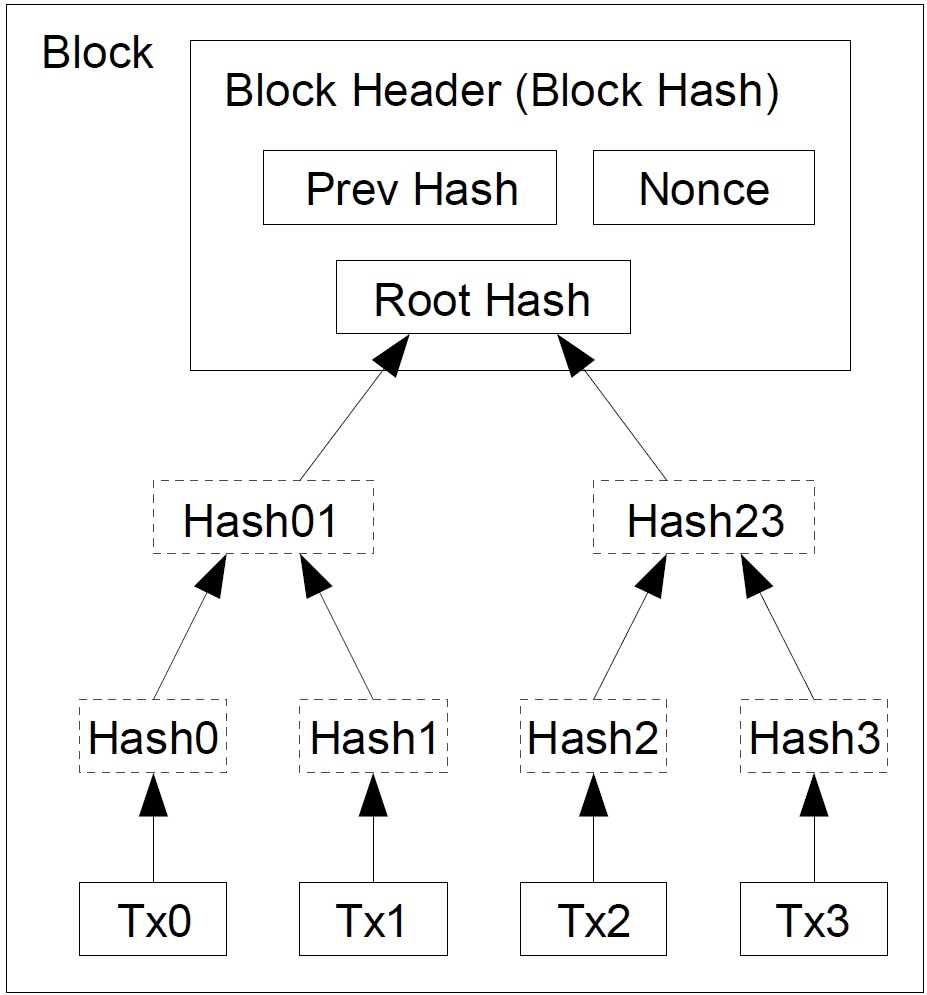
\includegraphics[width=120mm,scale=0.5]{figs/blockdisected}
	\caption{Transactions Hashed in a Merkle Tree \cite{paper:001}}
	\label{fig:blockdisected}
\end{figure}
\begin{figure}[h]
	\centering
    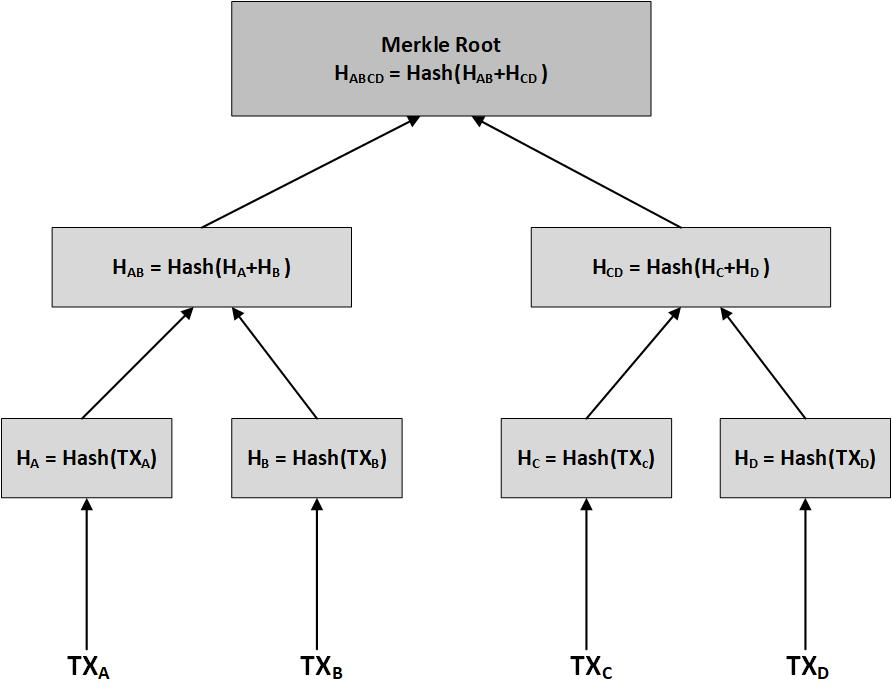
\includegraphics[width=160mm,scale=0.5]{figs/mtree}
	\caption{Constructing a Merkle Tree, adapted from \cite{andy_mb}}
	\label{fig:mtree}
\end{figure}
\clearpage

\subsection{Consensus Mechanisms - Mining} \label{Mining}
Electronic coins are defined as a chain of digital signatures that serves to establish ownership. In order for Alice to transfer one coin to Bob she must sign the hash of a previous transaction and the public key of the next owner i.e. Bob. Anyone can verify the chain of ownership by verifying signatures. This process only verifies that Alice was in possession of the coin at some point in time, it does not guarantee that Alice did not try to spend the same coin more than once.  Therefor a mechanism is needed that guarantees that any previous owner (Alice) did not sign any earlier transaction for transferring the same coin. The only way to verify this in a decentralize system is to announce all transactions and to have a mechanism to ensure that all participants agree on a single shared history or order of transactions. Payee (Bob) needs proof that at the time of each transaction, the majority of participants agreed that it was the first one \cite{paper:001}. The process which establishes consensus among all participants is called Mining.
%%%%%%%%%%%%%%%%%%%%%%Extras%%%%%%%%%%%%%%%%%%%%%%%%%
%put the figure of digital coin from bitcoin white paper section transactions
\subsubsection{Mining}
Mining underpins bitcoin or blockchain’s security model. This process is a designed to guarantee security and integrity of the distributed ledger. It serves to protect the network from fraudulent transactions and double spend attacks i.e. spending the same coins twice. It is also the process by which new blocks are generated. Miners spend something of value like electricity in the form of computing power by running complicated algorithms (Proof of Work). They are rewarded by the network with block rewards or newly minted coins. It prevents bad actors or attackers from modifying the state of decentralized ledger against network rules. Attackers will need to control at least fifty-one percent of network hash rate to mount a successful attack. This is virtually impossible in a sufficiently decentralized network like Bitcoin or Ethereum. There are two main type of mining algorithms Proof-of-Work \ref{PW} and Proof-of-Stake \ref{PS}.
  
\subsubsection{Proof-of-Work} \label{PW}
It was proposed by Satoshi Nakamoto in the bitcoin white paper \cite{paper:001}as means for establishing consensus. Miners solve complicated mathematical problems to validate transactions. Pending transactions are batched into blocks and the miners compete with each other to calculate the hash of the block. The hash output of the block must start with specific number of leading zeroes in order to satisfy protocol rules. The exact number of leading zeroes depend upon the network difficulty and is adjusted automatically every 2016 block. This difficulty determines how easy or hard it is to find the output hash for a block. The function that calculates difficulty is determined by a moving average and targets average number of blocks per hour. If blocks are generated too fast, the difficulty increases and vice versa. This is done in order to compensate for increasing hardware speed and varying interests in running nodes. Proof-of-work protocols can be summarized in the following steps \cite{medium:001}.

\begin{itemize}
  \item Miners try to find the hash output for a block with a fixed number of leading zeroes. They do this by repeatedly changing part of the block called nonce and recalculating the hash output.
  \item First miner to solve the puzzle and find the hash broadcasts his solution or proof-of-work to the rest of the network.
  \item Upon receiving the solution other miners verify it to ensure that it is correct. Before they agree to add the it to the blockchain they verify all the transaction in the block to make sure they are valid.
  \item If majority of miners agree on the solution and agree to add the block to the blockchain than consensus is achieved.
\end{itemize}

\subsubsection{Proof-of-Stake} \label{PS}
Proof of Work algorithms require miners to solve complicated math problems to verify transactions and generate new blocks. This approach has some inherent disadvantages. It requires huge amounts of electricity to achieve consensus in large blockchain networks such as Bitcoin and Ethereum. Some estimates have put bitcoins annual energy consumption on the same level as countries likes Austria or Switzerland. POW operates on the basis of one CPU one vote model. This approach can lead to mining centralization by large mining pools and chip manufacturers. Proof of Stake is an alternative approach for reaching consensus and protecting from double spend attacks in a decentralized network. It solves many problems inherent to POW algorithms. It is defined as \textit{“Proof of Stake (PoS) is a category of consensus algorithms for public blockchains that depend on a validator's economic stake in the network”} \cite{ethwiki:006}. POS requires users or forgers as they are called to lock up their digital coins in an escrow to get a chance to validate new blocks. The deposited coins serve as collateral and an incentive for the forgers to behave honestly. If a forger approves fraudulent transaction they will lose the coins they staked and will be banned from participating in the block validation process in the future. The crux of POS systems is the fact that for any attack to be successful the attacker will need to own majority of the coins on the network. Therefore, the attacker will be the one most severely impacted by his own attack \cite{bitwiki:005}. This serves as a huge deterrent against any potential bad actors. Block validators are incentivized with block rewards (combination of Tx fees and coins). They are selected by the network in a pseudo – random selection process based on a combination of factors. Selecting forgers solely on the size of their stake will hugely benefit the rich miners making the rich even more richer. There are several methods to avoid these problems two of which are given below. \cite{medium:002}\cite{misc:001}

\textbf{Coin Age based Selection:}
This method choses validators based on how long their coins have been staked for or the ‘coin age’ of their stake. The coin age is calculated by multiplying the size of a validators stake with the number of days the coins have been held in escrow. Once a validator generates a block their coin age is reset and they have to wait a fixed amount of time before they can be selected to validate another block \cite{misc:001}.

\textbf{Randomized Block Selection:}
This method choses validators based on a combination of lowest hash value and the size of their stake \cite{misc:001}.

%%%%%%%%%%%%%%%%%%%%%%Extras%%%%%%%%%%%%%%%%%%%%%%%%%
%\subsubsection{Delegated Proof of stake}
%\subsection{Full Nodes}
%\subsection{Transaction Finality}
%mention how finality can impact confirmation times and how it might impact any %potential supply chain management app.
%https://medium.com/coinmonks/blockchain-finality-pow-and-pos-35915a37c682
\subsection{Challenges:Scaling Debate}\label{scaling}
Blockchain technology is still in its infancy. It is a novel idea to solve several interesting problems in a trustless and decentralized manner, however in order to compete with existing centralized platforms it needs to be able to scale to handle millions of transactions per second. Let us consider the most common use case where the blockchain is used for making payments or to transfer assets between users. Bitcoin can on average perform 3 to 4 transactions per second while Ethereum can handle up to 20 transactions per second. Compare this to Visa which on average handled over 1100 transactions per second in 2016 and has an estimated capacity to perform up to 100000 transactions in a second \cite{medium:003}. Transaction speed measured in TPS is an important to metric to measure the performance of any financial system. During 2016 and 2017 major blockchain networks saw enormous growth in their user base. This caused exponential increase in transaction volume resulting in congested networks which caused huge delays in transaction confirmations [\ref{fig:mct}]. This had a domino effect on transaction fees as well, causing them to sky rocket as miners are incentivized to pick transactions with higher fees to mine first. The long confirmation delays coupled with high transactions fees caused many organizations and vendors to stop accepting bitcoins. There was an interesting case in 2017 when a conference held to promote the benefits of bitcoin and blockchain stopped accepting bitcoins as a mode of payment due precisely due to reasons outlined earlier.  The scaling problem is further amplified in smart contract platforms like Ethereum[\ref{eth}] which aim to be a hub for large scale decentralized applications or Dapps. Most existing and proposed Dapps use mircotransaction (MTX) as part of their business model. “Microtransactions are a business model where users can purchase virtual goods via micropayments” \cite{wiki:007}. In order to efficiently run such applications Ethereum needs a way to effectively handle $\mu$-transactions. In most cases these transactions need to be executed immediately and cannot wait for long block confirmation times. According to some estimates using current mechanisms “we’re roughly 250x off being able to run a 10m user app and 25,000x off being able to run Facebook on chain” \cite{medium:003}.  This requires exponential increase in transactions per second for blockchain to become a viable alternative to centralized solutions.
\begin{figure}[h]
	\centering
    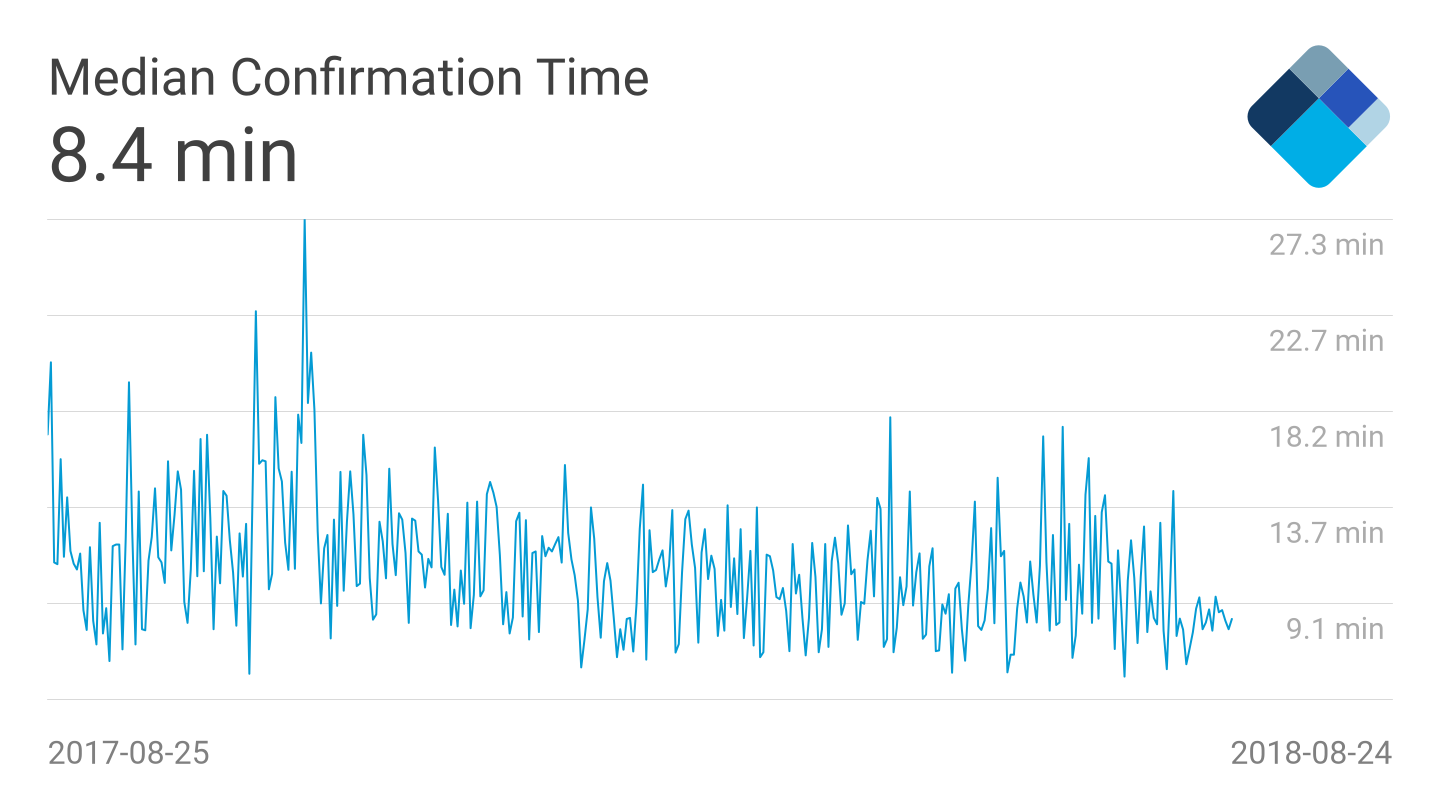
\includegraphics[width=120mm,scale=1]{figs/median-confirmation-time}
	\caption{Median confirmation times for BTC transactions \cite{fig:001}}
	\label{fig:mct}
\end{figure}
\clearpage

\subsubsection{Increasing Blocksize}
Transactions are grouped into blocks before they are verified. POW consensus rules require that there is some distance between successive blocks so that each verified block is successively incorporated by a majority of nodes in their copy of the ledger. This means that roughly only one block is generated every ten minutes \cite{paper:001}. In addition, some blockchains like Bitcoin have placed an upper limit on the size of each block. Currently for bitcoin the block size limit is 1 megabyte. One suggestion is to simply increase the block limit to allow more transactions to be verified at any given time.  This solution however has many problems first of all increasing block size results in only a linear increase in transactions per second. Secondly, it will adversely impact the decentralization of the network. Larger blocks require higher computational power to process each block and also drastically impact the size of the distributed ledger. This leads to more centralization as not everyone can afford the equipment required to successfully mine new blocks \cite{medium:006}. 
\subsubsection{Payment Channels - Lightning Network}
An alternative solution is to use Layer - 2 transaction networks. Lightning network is bitcoins proposed solution for the scaling problem. Lightning network is defined as \textit{“A decentralized system for instant, high-volume micropayments that removes the risk of delegating custody of funds to trusted third parties”} \cite{paper:002}. It advocates using payment channels to handle transactions off chain. \textit{“Payment Channel is class of techniques designed to allow users to make multiple Bitcoin transactions without committing all of the transactions to the Bitcoin block chain. In a typical payment channel, only two transactions are added to the block chain but an unlimited or nearly unlimited number of payments can be made between the participants”} \cite{bitwiki:006}.  Payment channels are essentially multi-signature bitcoin addresses. In order to spend funds from the channel both parties must sign off on the transaction agreeing to the new balance of the channel. The new balance is stored as the most recent transaction in the channel. Simply put, a payment channel is a smart contract on the bitcoin blockchain which is mostly executed off-chain after creation. In an ideal case, the only two transactions that go on the block chain are the ones for opening and closing a channel \cite{misc:011}. Participants of the channels can make unlimited instant transactions to each other while the channel is open. \textit{“Security is enforced by blockchain smart-contracts without creating an on-blockchain transaction for individual payments. Payment speed is measured in milliseconds to seconds”} \cite{paper:002}. This enables users to make off chain payments with confidence. If anything goes wrong blockchain can cryptographically verify the terms of the smart contract and enforce them on-chain \cite{bitwiki:006} \cite{misc:012}.
\clearpage
\subsubsection{Sidechains}
Sidechain is a blockchain that runs parallel to the main blockchain. It extends the functionality of the main chain enabling decentralize transfer of assets and tokens between the two chains. They allow coins to be moved between two separate blockchains. Tokens from the main chain can be securely moved to the sidechain and used in these chains. The token transfer takes places at a fixed predetermined rate \cite{misc:013}. In order to transfer main chain assets to a side chain they are sent to a special address on the main chain. Once this transaction is verified a confirmation is broadcast in the sidechain enabling the network to assign equivalent assets to the users account in the sidechain \cite{paper:004}. They can help with blockchain scaling as they can take some of the pressure of the main chain. Developers can design specialized sidechains to run their Dapps more efficiently while still taking advantage of security and decentralization provided by the mainchain. Sidechains are implemented using a Two – way peg as shown in figure [\ref{fig:SC}].
\vspace*{2cm}
\begin{figure}[h]
	\centering
    \includegraphics[width=160mm,scale=1]{figs/sidechain}
	\caption{Two way Pegged Sidechain }
	\label{fig:SC}
\end{figure}

\textbf{RootStock RSK SideChain}
It is a sidechain to bitcoin. It is Two-way pegged to bitcoin. RSK code aims to be backwards compatible to Ethereum i.e. code can be written in solidity or serpent and can be used on Ethereum. RSK aims to be a platform for decentralized applications and smart contracts on bitcoin. Miners are incentivized to mine smart contracts on RSK by rewarding them with bitcoins. Bitcoin miners can simultaneously mine both blockchains and rewarded through a process called “merge-mining”. Rootstock has its own version of Ethereum virtual machine (EVM). Currently the developers are working on what is called a federated peg which is essentially a system of notaries and a Multisignature exit address. The developers aim to go from federated peg to a two-way pegged system based on Simplified Payment Verification (SPV) \cite{andy_mb} \cite{paper:005}. 

\textbf{Federated peg:} is a system consisting of a set of notaries and a Multisignature exit address. When you send funds to this exit address you can create an SPV proof on RSK sidechain. This SPV proof allows you to convert the locked bitcoins in the federated address into bitcoins on rootstock sidechain. This is done automatically. However, moving funds from RSK back to bitcoin requires collaboration of federators. Basically a smart contract acts as bridge master and controls all unspent transaction outputs. This contract broadcasts a transaction to federators by using a log message. On receiving this message, federators send signatures to bridge master who combines all these signatures in to a fully signed transaction. This signed transaction is broadcast to RSK blockchain where any user can put this transaction onto bitcoin blockchain. This unlocks bitcoins on the bitcoin blockchain \cite{paper:005}.


